\documentclass[a4paper]{article}

\usepackage{onecolpceurws}
\usepackage[usenames,dvipsnames,table]{xcolor}
\usepackage[T1]{fontenc}
\usepackage{geometry}
\usepackage{paralist}
\usepackage{graphicx}
\usepackage[cache]{minted}
\usepackage{url}
\usepackage[utf8]{inputenc}
\usepackage{paralist}
\usepackage{amstext}
\usepackage{amsfonts}
\usepackage{xspace}
\usepackage{todonotes}
\usepackage{hyperref}

% \usepackage[skip=0pt]{caption}
% \usepackage{setspace}
% \setstretch{0.96}

% \hypersetup{
%   colorlinks,
%   breaklinks,
%   bookmarksnumbered=true,
%   pdftitle={Solving the TTC'16 Class Responsibility Assignment Case Study with SIGMA and Multi-Objective Genetic Algorithms},
%   pdfauthor={Filip Křikava},
%   linkcolor=Blue,
%   citecolor=BrickRed,
%   filecolor=Blue,
%   urlcolor=Blue
%   }

\renewcommand{\ttdefault}{pcr}

\newcommand{\SIGMA}{\textsc{Sigma}\xspace}
\newcommand{\FIXML}{FIXML\xspace}
\newcommand{\TTC}{TTC'16\xspace}
\newcommand{\Ie}{\emph{i.e.}\xspace}
\newcommand{\Eg}{\emph{e.g.}\xspace}
\newcommand{\Etal}{\emph{et al.}\xspace}
\newcommand{\Cf}{\emph{cf.}\xspace}

\newcommand{\Paragraph}[1]{\vspace*{2mm} \noindent \textbf{#1.}}
\newcommand{\Todo}[1]{\todo[inline]{#1}}
\renewcommand{\Todo}[1]{}

\newminted{scala}{fontsize=\fontsize{8}{8},numbersep=5pt,frame=lines,framesep=2mm}
\newminted{bash}{fontsize=\fontsize{8}{8},numbersep=5pt,frame=lines,framesep=2mm}

\newcommand{\Scala}[1]{\mintinline{scala}{#1}}

\title{Solving the \TTC Class Responsibility Assignment Case Study with SIGMA and Multi-Objective Genetic Algorithms}

\author{Filip Křikava\\ Faculty of Information Technology\\ Czech Technical University\\ \texttt{filip.krikava@fit.cvut.fr}}
\institution{}

\begin{document}
\maketitle

\begin{abstract}
In this paper we describe a solution for the \emph{Transformation Tool Contest 2016} (\TTC) Class Responsibility Assignment (CRA) case study using \SIGMA, a family of Scala internal \emph{Domain-Specific Languages} (DSLs) that provides an expressive and efficient API for model consistency checking and model transformations.
Since the Class Responsibility Assignment problem is a search-based problem, we base our solution on multi-objective genetic algorithms.
Concretely, we use NSGA-III and SPEA2 to minimize the coupling between classes' structural features and to maximize their cohesion.
\end{abstract}

%!TEX root = ttc16-cra-sigma.tex

% \enlargethispage{10mm}

\section{Introduction}
\label{sec:Introduction}

%% Overview
In this paper we describe our solution for the \TTC Class Responsibility Assignment (CRA) case study~\cite{Fleck2016} using the \SIGMA~\cite{Krikava2014}.
The goal of this case study is to find high-quality class diagrams from existing responsibility dependency graphs (RDG).
The RDGs only contain a set of methods and attributes with functional and data relationships among them.
The CRA problem is essentially about deciding where the different responsibilities in the form of class structural features (\Ie operations and attributes) belong and how objects should interact by using those operations~\cite{bowman2010solving}.
Since the design space of all possible class diagrams grows exponentially with the size of the RDG model~\cite{Fleck2016} (\Ie the number of structural features), the problem could be solved using search-based optimization techniques~\cite{coello2007evolutionary}.
Concretely, the use of multi-objective genetic algorithms seems to provide an efficient solution for the CRA problem as demonstrated by Bowman~\Etal~\cite{bowman2010solving}.

In this paper, we therefore present a solution to the CRA problem using \SIGMA and multi-objective genetic algorithms.
We use \SIGMA to transform the input RDG diagram into a search-based problem which is then solved by a genetic algorithm.
In the implementation we use NSGA-III and SPEA2 algorithms from the MOEA framework\footnote{\url{http://www.moeaframework.org/}}.
The MOEA Framework is a free and open source Java library for developing and experimenting with multi-objective evolutionary algorithms (MOEAs) and other general-purpose multi-objective optimization algorithms~\cite{moea}.

%% Scala
\SIGMA is a family of Scala\footnote{\url{http://scala-lang.org}} internal DSLs for model manipulation tasks such as model validation, model to model (M2M), and model to text (M2T) transformations.
Scala is a statically typed production-ready \emph{General-Purpose Language} (GPL) that supports both object-oriented and functional styles of programming.
It uses type inference to combine static type safety with a \emph{``look and feel''} close to dynamically typed languages.
Furthermore, it is supported by the major integrated development environments bringing EMF modeling to other IDEs than traditionally Eclipse (the solution was developed in IntelliJ IDEA\footnote{\url{https://www.jetbrains.com/idea/}}).

%% SIGMA
\SIGMA DSLs are embedded in Scala as a library allowing one to manipulate models using high-level constructs similar to the ones found in the external model manipulation DSLs.
The intent is to provide an approach that developers can use to implement many of the practical model manipulations within a familiar environment, with a reduced learning overhead as well as improved usability and performance.
The solution is based on the \emph{Eclipse Modeling Framework} (EMF)~\cite{EMF}, which is a popular meta-modeling framework widely used in both academia and industry, and which is directly supported by \SIGMA.

In this particular \TTC case study, the main problem is in solving an optimization problem rather than a transformation problem.
\SIGMA is therefore only used to transform input RDG model into an optimization problem and to transform the problems' solutions into class diagrams.

%% Organization
The complete source code is available on Github\footnote{\url{https://github.com/fikovnik/ttc16-cra-sigma}}.
In the Appendix~\ref{sec:InstallLocally} and~\ref{sec:InstallSHARE} we provide steps how to install it locally as well as how to run it on the SHARE environment.
%!TEX root = ttc16-cra-sigma.tex

\section{Solution Description}
\label{sec:SolutionDescription}

The core of this case study is to transform a RDG model into a high-quality class digram (\Cf Figure~\ref{fig:Metamodel}).

\begin{figure*}[h!tb]
  \centering
  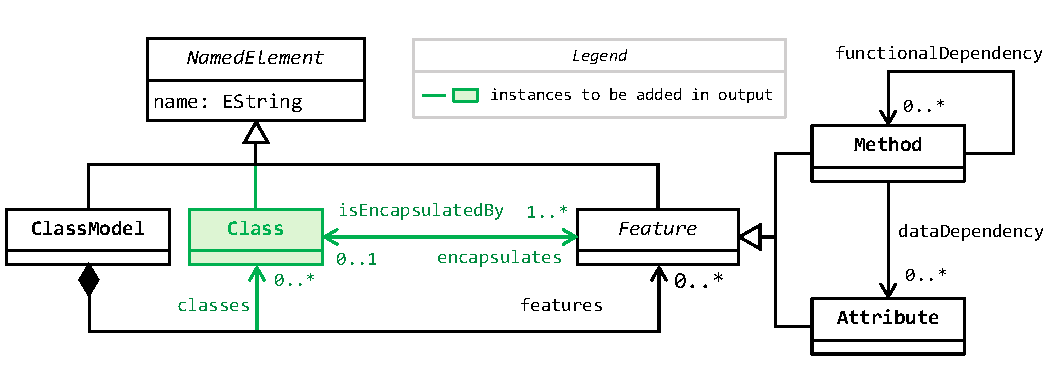
\includegraphics[width=.8\textwidth]{figures/metamodel.pdf}
  \caption{RDG and class model metamodel}
  \label{fig:Metamodel}
\end{figure*}

To consider the quality of a class digram, two common software engineering metrics are used: \emph{coupling} (the number of external dependencies) and \emph{cohesion} (the number of internal dependencies).
The two metrics can be further combined in one, single quality metric called \emph{CRA-Index}, which simply subtracts the coupling from cohesion.
The case study authors provide a set of utility functions that can compute all these metrics from a class digram instance and therefore we do not need to concern ourselves by their precise definitions.

The outline of the solution proposed in this paper is as follows:

\begin{compactenum}
  \item Loads the input RDG model from a given XMI file.
  \item Transforms the RDG model into MOEA problem instance.
  \item Runs the MOEA solver using either NSGA-III or SPEA2 algorithms.
  \item From the possible solutions (which are part of a Pareto optimal front~\Cf below), selects the one with the highest CRA-Index.
  \item Transforms the selected solution into class digram.
  \item Saves the resulting class diagram into XMI file.
\end{compactenum}

\subsection{Transformations}

An optimization problem defines a search space, or the set of possible solutions together with one or more objective functions.
In our case the search space are all the valid class diagrams that can represent given RDG model.
The objectives are:
%
\begin{inparaenum}[(1)]
\item to minimize coupling, and
\item to maximize cohesion.     
\end{inparaenum}

The functions that compute coupling and cohesion ratios from a class diagram are part of the case study description.
What remains is to find the way how to represent the RDG model as a vector of variables that can be used in a evolutionary algorithm to find a solution.
We use a simple integer vector where the index corresponds to the feature index in the input RDG model and the value corresponds to the index of a class in the resulting class diagram.
The bound of each vector element is bounded between 0 and the number of features $- 1$ (since we use 0-based indexing).
For example, a vector $\left( 3, 5, \dots \right)$ represents a solution in which first feature belongs to fourth class, second feature to sixth class, and so on and so forth.
Figure~\ref{fig:SolutionOverview} shows a further example of this representation on the example input/output model pair from the case description~\cite{Fleck2016}.

\begin{figure}[h!tb]
  \centering
  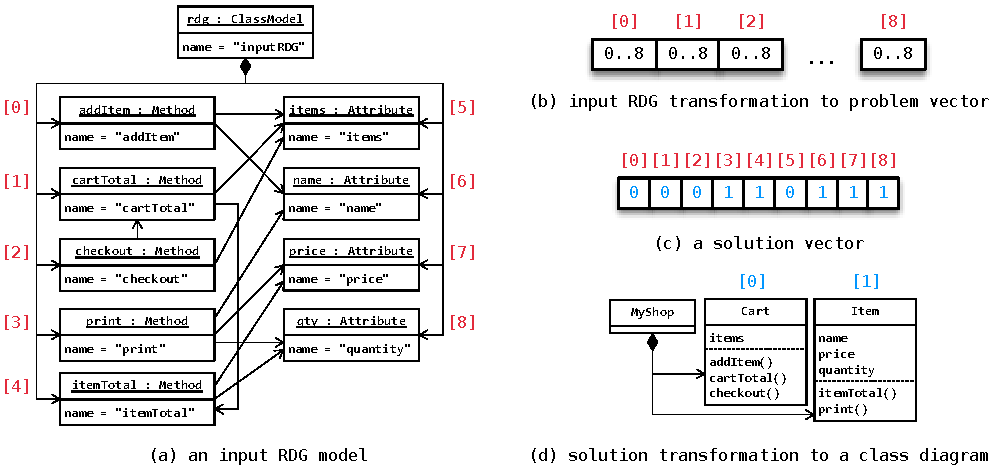
\includegraphics[width=.9\columnwidth]{figures/solution-overview.pdf}
  \caption{Example of the Solution}
  \label{fig:SolutionOverview}
\end{figure}

The advantage of this representation is that it can be easily mapped to MOEA decision variables.
Also, each feature will always be assigned to (encapsulated by) some class.
Therefore, the second validation constraint \emph{all features provided in the input model must be encapsulated by a class}, will be always satisfied without any additional logic.

\enlargethispage{5mm}

Concretely, in the MOEA framework, we have created a \texttt{Problem} class, called \texttt{CRAProblem}.
The integer vector is used to define the decision variables, their types (\Ie integers) and bounds (\Ie $0\dots\text{number of features}-1$).
The number of decision variables corresponds to the number of features in the input RDG model.
The number of objectives is always two, the first one for coupling and the second one for cohesion.
The method instantiating new solution instances looks as follows:
%
\begin{scalacode}
override def newSolution() = {
  val s = new Solution(numVars, numObjs)
  (0 until numVars) foreach (x => 
    s.setVariable(x, newInt(0, numVars - 1))
  )
  s // return the new instance
}
\end{scalacode}

Next to providing a method to instantiate new instances of solutions for the problem, we need to also define the evaluation of a solution to compute the objectives.
This involves two steps:
%
\begin{inparaenum}[(1)]
  \item transforming the solution into a class diagram
  \item using the provide \texttt{calculateCoupling} and \texttt{calculateCohesion} utility functions to compute the metrics.
\end{inparaenum}
%
In code this is implemented as:
%
\begin{scalacode}
override def evaluate(s: Solution) = {
  // transformation
  val m = solutionToClassModel(initModel, s)
  // minimize coupling
  s.setObjective(0,calculateCoupling(m))
  // maximize cohesion
  s.setObjective(1,-calculateCohesion(m))
}
\end{scalacode}
%
The negation of the cohesion ratio is due to the fact that MOEA only works on minimization problems and thus we need to negate the objective value to convert from maximization into minimization.
The code that does the transformation is shown in Listing~\ref{mnt:SolutionTransformation}.
This is the main code that uses \SIGMA.

\begin{listing}[!ht]
\begin{scalacode}
def solutionToClassModel(
  initModel: ClassModel, 
  s: Solution) = {

  // create a new model as a copy
  // of the input one
  val m = initModel.sCopy
  // get problem vector (v: Array[Int])
  val v = EncodingUtils.getInt(solution)
  // create new classes
  val classes = (0 to v.max) map (x => 
    Class(name = s"Class $x")
  )

  // assignment
  v.zipWithIndex.foreach {
    case (cIdx, fIdx) => 
      m.features(fIdx)
       .isEncapsulatedBy = classes(cIdx)
  }

  // add non-empty classes
  m.classes ++= classes filter (x => 
    !x.getEncapsulates.isEmpty
  )
  m
}
\end{scalacode}
\caption{Solution transformation}
\label{mnt:SolutionTransformation}
\end{listing}

Finally, we define a new type, \texttt{Solver}, which is a function $RDG \rightarrow ClassDiagram$.
The solver is responsible
%
\begin{inparaenum}[(1)]
  \item to find the Pareto optimal front of all possible solutions (subject to solver configuration), and
  \item to select the solution from that set which has the highest CRA-Index.
\end{inparaenum}
The Pareto optimal front refers to optimal solutions whose corresponding vectors are non-dominated by any other solution vector~\cite{bowman2010solving} and it can be found by MOEA \texttt{Executor}.
For example using the NSGA-III algorithm, we find the non-dominated vector as:
%
\begin{scalacode}
new Executor()
  .withProblemClass(
    classOf[CRAProblem], 
    initModel)
  .withAlgorithm("NSGAIII")
  .withProperty("populationSize", 64)
  .withMaxEvaluations(10000)
  .run()
\end{scalacode}
%
The individual solutions in this vector are first converted to the class model using Listing~\ref{mnt:SolutionTransformation} and we use the given \texttt{calculateCRA} function to find the highest CRA.
To have a better chance to find a good solution, we run each algorithm 10 times.
The properties of each algorithm are defined based on the suggestion by Bowman~\Etal~\cite{bowman2010solving}.

The code is organized into three classes in \texttt{src/main/scala} folder:
%
\begin{compactitem}[---]
  \item \texttt{CRAProblem} defines the CRA problem in terms of MOEA problem,
  \item \texttt{Solvers} preconfigures the two used algorithms for the finding the non-dominated solution vector, and finally
  \item \texttt{Main} that assembles the solution together into an executable application.
\end{compactitem}
%!TEX root = ttc16-cra-sigma.tex

\section{Evaluation}
\label{sec:Evaluation}
\enlargethispage{10mm}

In this section we provide an evaluation of our solution following the categories given by the case study description.
We leave the complexity and flexibility characteristics to be evaluated by reviewers.
All the presented results are based on the NSGA-III algorithm. 
More results are provided on the github page.

\Paragraph{Completeness \& Correctness}
The solution always converts a valid input RDG into a class model.
The three constraints that were imposed by the solution description are solved as follows:
%
\begin{compactitem}[---]
  \item \emph{Every class must have a unique name.} 
  The new classes are created in a loop that iterates over a number range.
  Part of the class name is the iteration variable and thus it must be always unique.
  \item \emph{All features provided in the input model must be encapsulated by a class.} 
  This has been already explained in the previous section.
  This is a property of the problem mapping we have chosen.
  \item \emph{There cannot be any empty classes.}
  We explicitly filter out empty classes.
\end{compactitem}

\Paragraph{Optimality and Performance}
The following table shows the cohesion and coupling rations, the resulting CRA-Index as well as the completion time from the SHARE environment\footnote{These are the initial results submitted for the competition. Improved result obtained after a better use of parallelism and better crossover and mutation ratios are available at \url{https://github.com/fikovnik/ttc16-cra-sigma}}:
\begin{center}
\begin{tabular}{crrrr}
\hline
\textbf{Input} & \textbf{Cohesion} & \textbf{Coupling} & \textbf{CRA} & \textbf{Time {[}s{]}} \\ \hline
A           & 4        & 1        & 3       & 19.17    \\
B           & 6.5      & 2.5      & 4       & 34.78    \\
C           & 6.37     & 3.63     & 2.74    & 72.53    \\
D           & 4.83     & 7.94     & -3.11   & 300.49   \\
E           & 7.38     & 17.99    & -10.60  & 1110.74  \\
F           & 9.85     & 44.74    & -34.88  & 6289.75  \\ \hline
\end{tabular}
\end{center}

%!TEX root = ttc16-cra-sigma.tex

% \vspace*{-3mm}
% \enlargethispage{7mm}


% \section{Conclusion}
% \label{sec:Conclusion}


% This case study provides a good illustration for some of the capabilities of an internal DSL approach to model querying and transformation.

% Say something about Scala itself











\bibliographystyle{alpha}
\bibliography{references.bib}

\appendix

%!TEX root = ttc16-cra-sigma.tex

\section{Install and Run Locally}
\label{sec:InstallLocally}

The only requirements for running the solution is to have \texttt{git} and \texttt{sbt}\footnote{simple-built-tool \Cf \url{http://www.scala-sbt.org/}} tools installed.
To reproduce the benchmark simply execute these steps in a command line:

\begin{bashcode}
$ git clone \
  https://github.com/fikovnik/ttc16-cra-sigma
$ cd ttc16-cra-sigma
$ ./build.sh
$ ./run.sh
\end{bashcode}

\section{Install and Run on SHARE}
\label{sec:InstallSHARE}

On the share environment we provide ready to be run solution. Simply log into the SHARE VM \texttt{remoteArchLinux64-TTC16\_SIGMA} with \texttt{ttcuser/ttcuser} as user name/password and run the following:

\begin{bashcode}
$ cd ttc16-cra-sigma
$ ./run.sh
\end{bashcode}

\end{document}
